\documentclass{article}
\usepackage[utf8]{vietnam}
\usepackage[14pt]{extsizes}
\usepackage{amsmath,amsfonts,amsthm}
\usepackage{geometry}
\usepackage{mathrsfs}
\usepackage{graphicx}
\usepackage{float}
 \geometry{
 a4paper,
 total={170mm,257mm},
 left=20mm,
 top=20mm,
}
\usepackage{enumitem}
\title{Đáp án đề số 1 năm 2025}
\begin{document}
\maketitle
\textit{\textbf{Lưu ý:} Đây chỉ là đáp án tham khảo do mình tự soạn dựa trên quá trình làm bài ngày hôm nay chứ không phải là đáp án chính thức. Nếu có lỗi sai cần sửa các bạn có thể liên hệ với mình qua email tinvu1309@gmail.com. Cảm ơn các bạn!}
\section*{Đề 1}
\subsection*{1. Tính năng lượng của tín hiệu $x[n]=\sum_{k=0}^{+\infty}2^{-k}\delta[n-3k]$}
Câu này các bạn chỉ cần vẽ tín hiệu $x[n]$ ra là có thể tính được năng lượng của nó ngay.
\begin{figure}[H]
    \centering
    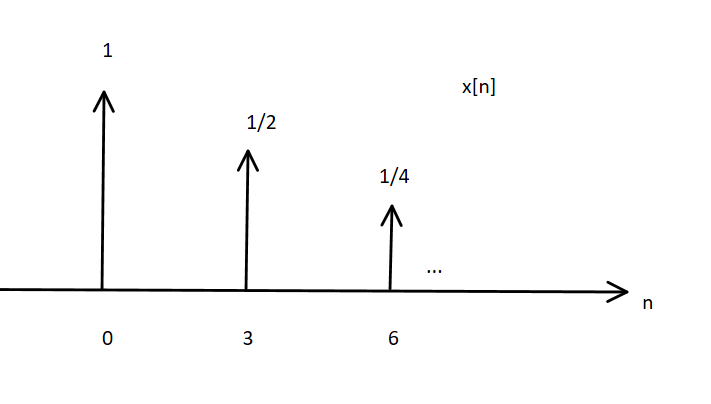
\includegraphics[width=0.8\textwidth]{1.png}
    \caption{Tín hiệu $x[n]$}
    \label{dongco}
\end{figure}
Vậy ta có 
\begin{equation*}
\begin{split}
E=\sum_{n=-\infty}^{+\infty}|x[n]|^{2}&=1+\left(\frac{1}{2}\right)^{2}+\left(\frac{1}{4}\right)^{2}+...=\left(\frac{1}{2}\right)^{0}+\left(\frac{1}{2}\right)^{2}+\left(\frac{1}{2}\right)^{4}+...\\&=\frac{1}{1-\left(\frac{1}{2}\right)^{2}}=\frac{4}{3}
\end{split}
\end{equation*}
\subsection*{2. Khảo sát các đặc trưng của hệ thống liên tục được biểu diễn bởi quan hệ vào - ra sau $y(t)=e^{-2t}x(t)$}
\begin{itemize}
    \item Không nhớ: Dễ thấy hệ thống này không nhớ do giá trị của $y(t)$ chỉ phụ thuộc vào thời điểm $t$ hiện tại, từ đó ta kết luận đây cũng là hệ thống nhân quả.
    \item Tuyến tính: Giả sử ta có hai tín hiệu đầu vào $x_{1}(t)$ và $x_{2}(t)$, sau khi cho qua hệ thống ta thu được hai tín hiệu đầu ra tương ứng:
    $$y_{1}(t)=e^{-2t}x_{1}(t)$$ $$y_{2}(t)=e^{-2t}x_{2}(t)$$
    Ta xét tín hiệu $x_{3}(t)=Ax_{1}(t)+Bx_{2}(t)$ ($A, B$ là các hằng số tùy ý), sau khi cho qua hệ thống, ta cũng thu được đầu ra:
    $$y_{3}(t)=e^{-2t}x_{3}(t)=e^{-2t}(Ax_{1}(t)+Bx_{2}(t))=Ay_{1}(t)+By_{2}(t)$$
    Vậy ta kết luận đây là hệ thống tuyến tính.
    \item Bất biến: Giả sử ta có hai tín hiệu đầu vào $x_{1}(t)$ và $x_{2}(t)=x_{1}(t-t_{0})$ ($t_{0}$ là hằng số), khi cho qua hệ thống, ta cũng thu được hai tín hiệu đầu ra tương ứng.
    $$y_{1}(t)=e^{-2t}x_{1}(t)$$
    $$y_{2}(t)=e^{-2t}x_{2}(t)=e^{-2t}x_{1}(t-t_{0})\neq y_{1}(t-t_{0})=e^{-2(t-t_{0})}x_{1}(t-t_{0})$$
    Vậy ta kết luận đây là hệ thống không bất biến
    \item Ổn định: Giả sử $|x(t)|<B$, thế nhưng tại thời điểm $t\to-\infty$ thì $y(t)\to+\infty$, nên hệ thống này không ổn định.
\end{itemize}
\subsection*{3. Xét một hệ thống tuyến tính bất biến liên tục và ổn định được biểu diễn bởi phương trình vi phân $y''(t)+y'(t)-12y(t)=x'(t)$}
\subsubsection*{(a) Tính đáp ứng biên độ $|H(\omega)|$ của hệ thống tại tần số $\omega=3$ (rad/s)}
Sử dụng biến đổi Laplace cho cả hai vế, ta có:
\begin{equation*}
    \begin{split}
    \mathscr{L}(y''(t)+y'(t)-12y(t))&=\mathscr{L}(x'(t))\\Y(s)(s^{2}+s-12)&=sX(s)
    \\\Rightarrow H(s)=\frac{Y(s)}{X(s)}&=\frac{s}{s^{2}+s-12}
    \end{split}
\end{equation*}
Giải phương trình tìm điểm cực, ta có $s=3$, $s=-4$, do hệ thống này ổn định nên ta có $\mathfrak{Re}(s)>-4$ (miền ROC chứa trục $\mathfrak{Im}$).
Khi hệ thống ổn định, ta có
$$H(\omega)=\frac{j\omega}{-\omega^{2}+j\omega-12}\Rightarrow |H(3)|=\frac{\sqrt{2}}{10}$$
\subsubsection*{(b) XÁc định đáp ứng xung của hệ thống}
\begin{equation*}
    \begin{split}
        h(t)&=\mathscr{L}^{-1}\left(\frac{s}{s^2+s-12}\right)=\mathscr{L}^{-1}\left(\frac{s}{(s-3)(s+4)}\right)=\mathscr{L}^{-1}\left(\frac{A}{s-3}+\frac{B}{s+4}\right)\\&=\mathscr{L}^{-1}\left(\frac{3}{7}.\frac{1}{s-3}+\frac{4}{7}.\frac{1}{s+4}\right)=\left(\frac{3}{7}e^{3t}+\frac{4}{7}e^{-4t}\right)u(t)
    \end{split}
\end{equation*}
\subsubsection*{(c) Xác định đáp ứng của hệ thống với tín hiệu vào $x(t)=\sin{(3t)}-1$}
\begin{equation*}
    \begin{split}
        x(t)&=\sin{(3t)}-1=\frac{1}{2j}(e^{j3t}-e^{-j3t})-1\\
        \Rightarrow y(t)&=\sum H(\omega)x(t)=H(0)(-1)+H(3)\frac{1}{2j}e^{j3t}-H(-3)\frac{1}{2j}e^{-j3t}\\&=\left(-\frac{7}{100}-j\frac{1}{100}\right)e^{j3t}+\left(\frac{-7}{100}+j\frac{1}{100}\right)e^{-j3t}=\frac{-7}{50}\cos{3t}+\frac{1}{50}\sin{3t}
    \end{split}
\end{equation*}
\subsubsection*{(d) Xác định đáp ứng của hệ thống với tín hiệu vào $x(t)=e^{-4t}u(t-1)$}
Ý tưởng của bài này đó là ta cần phải áp dụng công thức khai triển Laplace cùng với tính chất để tìm ra được $X(s)$ và $y(t)$. Đầu tiên ta xét 
$$\mathscr{L}(e^{-4t}u(t))=\frac{1}{s+4}$$
Áp dụng tính chất dịch thời gian $t_{0}$: $\mathscr{L}(x(t-t_{0}))=e^{-st_{0}}X(s)$, ta có:
\begin{equation*}
\begin{split}
\mathscr{L}(e^{-4(t-1)})u(t-1)=\frac{e^{-s}}{s+4}\Rightarrow X(s)=\mathscr{L}(e^{-4t}u(t-1))=\frac{e^{-s-4}}{s+4}
\end{split}
\end{equation*}
Vậy ta có:
$$Y(s)=H(s)X(s)=\frac{se^{-s-4}}{(s+4)(s^2+s-12)}$$
Đầu tiên ta sẽ xử lý phân thức 
$$\frac{s}{(s+4)(s^2+s-12)}=\frac{A}{s+4}+\frac{B}{(s+4)^2}+\frac{C}{s-3}$$
Các bạn dùng Casio giải hệ phương trình thì sẽ tính được các hệ số $A=\frac{-3}{49}, B=\frac{4}{7}, C=\frac{3}{49}$
.Vậy ta có:
\begin{equation*}
\begin{split}
\mathscr{L}^{-1}\left(\frac{s}{(s+4)(s^2+s-12)}\right)&=\mathscr{L}^{-1}\left(\frac{-3}{49}.\frac{1}{s+4}+\frac{4}{7}.\frac{1}{(s+4)^2}+\frac{3}{49}.\frac{1}{s-3}\right)\\
&=\left(\frac{-3}{49}e^{-4t}+\frac{4}{7}te^{-4t}+\frac{3}{49}e^{3t}\right)u(t)
\end{split}
\end{equation*}
Ta dễ dàng suy ra:
\begin{equation*}
\begin{split}
y(t)&=\mathscr{L}^{-1}(Y(s))=\mathscr{L}^{-1}\left(\frac{se^{-s-4}}{(s+4)(s^2+s-12)}\right)\\&=\left(\frac{-3}{49}e^{-4(t-1)}+\frac{4}{7}(t-1)e^{-4(t-1)}+\frac{3}{49}e^{3(t-1)}\right)e^{-4}u(t-1)\\&=\left(\frac{-3}{49}e^{-4t}+\frac{4}{7}(t-1)e^{-4t}+\frac{3}{49}e^{3t-7}\right)u(t-1)
\end{split}
\end{equation*}
\subsection*{4. Xét một hệ thống tuyến tính bất biến rời rạc nhân quả được biểu diễn bởi phương trình sai phân $y[n]+\frac{3}{2}y[n-1]-y[n-2]=x[n-1]$}
\subsubsection*{(a) Hệ thống có ổn định không, tại sao?}
\begin{equation*}
\begin{split}
\mathscr{Z}(y[n]+\frac{3}{2}y[n-1]-y[n-2])&=\mathscr{Z}(x[n-1])\\\Leftrightarrow Y(z)\left(1+\frac{3}{2}z^{-1}-z^{-2}\right)&=X(z).z^{-1}\\\Rightarrow H(z)=\frac{Y(z)}{X(z)}&=\frac{z^{-1}}{1+\frac{3}{2}z^{-1}-z^{-2}}
\end{split}
\end{equation*}
Giải phương trình đường tròn cực $1+\frac{3}{2}z^{-1}-z^{-2}=0$, ta có $|z|=2$ và $|z|=\frac{1}{2}$, do hệ thống nhân quả nên $|z|>2$ (không chứa đường tròn đơn vị $|z|=1$), vậy kết luận hệ thống này không ổn định.
\subsubsection*{(b) Xác định đáp ứng xung và đáp ứng tần số của hệ thống}
\begin{equation*}
\begin{split}
h[n]&=\mathscr{Z}^{-1}(H(z))=\mathscr{Z}^{-1}\left(\frac{z^{-1}}{1+\frac{3}{2}z^{-1}-z^{-2}}\right)=\mathscr{Z}^{-1}\left(\frac{A}{2-z^{-1}}+\frac{B}{\frac{1}{2}+z^{-1}}\right)\\&=\mathscr{Z}^{-1}\left(\frac{4}{5}.\frac{1}{2-z^{-1}}-\frac{1}{5}.\frac{1}{\frac{1}{2}+z^{-1}}\right)=\mathscr{Z}^{-1}\left(\frac{4}{10}.\frac{1}{1-\frac{z^{-1}}{2}}-\frac{2}{5}.\frac{1}{1+2z^{-1}}\right)\\&=\left[\frac{2}{5}\left(\frac{1}{2}\right)^{n}-\frac{2}{5}(-2)^{n}\right]u[n]
\end{split}
\end{equation*}
Hệ thống này không tồn tại đáp ứng tần số do nó không ổn định.
\subsubsection*{(c) Xác định đáp ứng tự nhiên $y_{0}[n]$ của hệ thống với điều kiện khởi tạo $y[-1]=1, y[-2]=-1$}
Ý hỏi này có hai cách làm là sử dụng phương trình sai phân và sử dụng biến đổi $Z$ một phía. Ở đây mình sẽ chữa cách giải bằng phương trình sai phân trước:
\\Khi không có tín hiệu đầu vào, ta có thể viết lại phương trình sai phân như sau:
$$y[n]+\frac{3}{2}y[n-1]-y[n-2]=0$$
Dễ thấy dạng nghiệm $y_{0}[n]=K_{1}\lambda_{1}^{n}+K_{2}\lambda_{2}^{n}$, giải phương trình đặc trưng $\lambda^{n}+\frac{3}{2}\lambda^{n-1}-\lambda^{n-2}=0$, ta tính được $\lambda_{1}=-2 ,\lambda_{2}=\frac{1}{2}$, thay vào điều kiện đầu $y[-1]=1, y[-2]=-1$, ta thu được $y_{0}[n]=\frac{-12}{5}(-2)^{n}-\frac{1}{10}\left(\frac{1}{2}\right)^{n}$
\\Với cách làm biến đổi $Z$ một phía, ta sẽ làm như sau:
\begin{equation*}
\begin{split}
\mathscr{UZ}{\left(y[n]+\frac{3}{2}y[n-1]-y[n-2]\right)}&=\mathscr{UZ}(x[n-1])\\
\Leftrightarrow \mathscr{Y}(z)+\frac{3}{2}\left(\mathscr{Y}(z)z^{-1}+y[-1]\right)-(\mathscr{Y}(z)z^{-2}+y[-1]z^{-1}+y[-2])&= \mathscr{X}(z)z^{-1}\\ \Leftrightarrow \mathscr{Y}(z)\left(1+\frac{3}{2}z^{-1}-z^{-2}\right)+\frac{3}{2}-z^{-1}+1&=\mathscr{X}(z)z^{-1}\\\Leftrightarrow \mathscr{Y}(z)=\frac{\mathscr{X}(z)z^{-1}}{1+\frac{3}{2}z^{-1}-z^{-2}}+\frac{z^{-1}-\frac{5}{2}}{1+\frac{3}{2}z^{-1}-z^{-2}}
\end{split}
\end{equation*}
Ta có $\mathscr{Y}(z)=\mathscr{Y}_{F}(z)+\mathscr{Y}_{0}(z)$, vậy ta cần phải tính:
\begin{equation*}
\begin{split}
y_{0}[n]&=\mathscr{UZ}^{-1}\left(\frac{z^{-1}-\frac{5}{2}}{1+\frac{3}{2}z^{-1}-z^{-2}}\right)=\mathscr{UZ}^{-1}\left(\frac{A}{2-z^{-1}}+\frac{B}{\frac{1}{2}+z^{-1}}\right)\\&=\mathscr{UZ}^{-1}\left(\frac{-6}{5}.\frac{1}{\frac{1}{2}+z^{-1}}+\frac{-1}{5}\frac{1}{2-z^{-1}}\right)\\&=\mathscr{UZ}^{-1}\left(\frac{-6}{5}.\frac{2}{1+2z^{-1}}-\frac{1}{10}.\frac{1}{1-\frac{z^{-1}}{2}}\right)=\left(\frac{-12}{5}(-2)^{n}-\frac{1}{10}\left(\frac{1}{2}\right)^{n}\right)u[n]
\end{split}
\end{equation*}
Cả hai đáp số tính bằng hai cách trên đều giống nhau, điểm khác nhau duy nhất nằm ở thừa số $u[n]$. Tất nhiên, cả hai đáp số đều đúng nhưng đáp số khi tính bằng phương trình sai phân tổng quát hơn và đúng với tất cả các trường hợp hệ thống nhân quả hay không, còn với cách tính bằng biến đổi $Z$ một phía (unilateral Z transform) thì chỉ đúng với trường hợp hệ thống nhân quả.
\subsubsection*{(d) Xác định đáp ứng của hệ thống với tín hiệu vào $x[n]=u[n]$ (khi không có điều kiện khởi tạo)}
Đề bài yêu cầu ta tìm $y_{F}[n]$, đầu tiên ta phải xác định dạng $y_{G}[n]$ (general solution - nghiệm tổng quát của hệ thống)
\\Ta xác định $y_{P}[n]$ như sau, giả sử dạng nghiệm của $y_{P}[n] = Au[n]$, ta có:
\begin{equation*}
\begin{split}
y[n]+\frac{3}{2}y[n-1]-y[n-2]&=x[n-1]\\\Leftrightarrow Au[n]+\frac{3}{2}Au[n-1]-Au[n-2]&=u[n-1]
\end{split}
\end{equation*}
Với $n\geq2$, ta có $u[n]=u[n-1]=u[n-2]=1$, nên ta tính được $A=\frac{1}{1+\frac{3}{2}-1}=\frac{2}{3}$.
\\Vậy ta có $y_{F}[n]=K_{1}(-2)^{n}+K_{2}(\frac{1}{2})^{n}+\frac{2}{3}$ với $n\geq2$. Ở đây, ta không được thay điều kiện $y[-1]=y[-2]=0$ vào luôn để tính mà bắt buộc phải tìm $y[2]$ và $y[3]$.\\
Với $n=0$, ta có:
$$y[0]+\frac{3}{2}y[-1]-y[-2]=u[-1]\Leftrightarrow y[0]=0$$
Với $n=1$, ta có:
$$y[1]+\frac{3}{2}y[0]-y[-1]=u[0]\Leftrightarrow y[1]=1$$
Với $n=2$, ta có:
$$y[2]+\frac{3}{2}y[1]-y[0]=u[1]\Leftrightarrow y[2]=\frac{-1}{2}$$
Với $n=3$, ta có:
$$y[3]+\frac{3}{2}y[2]-y[1]=u[2]\Leftrightarrow y[3]=\frac{11}{4}$$
Thay các kết quả $y[2]$ và $y[3]$ vào giải hệ phương trình, ta tính được $K_{1}=\frac{-4}{15}$ và $K_{2}=\frac{-2}{5}$.
\\Vậy ta có $y_{F}[n]=\frac{-4}{15}(-2)^{n}+\frac{-2}{5}(\frac{1}{2})^{n}+\frac{2}{3}$ với $n\geq2$., tức là:
$$y_{F}[n]=\left(\frac{-4}{15}(-2)^{n}+\frac{-2}{5}\left(\frac{1}{2}\right)^{n}+\frac{2}{3}\right)u[n-2]$$
Đối với cách làm biến đổi Z, ta cũng chỉ làm đơn giản như sau:
\begin{equation*}
\begin{split}
y_{F}[n]&=\mathscr{UZ}^{-1}\left(\frac{\mathscr{X}(z)z^{-1}}{1+\frac{3}{2}z^{-1}-z^{-2}}\right)=\mathscr{UZ}^{-1}\left(\frac{z^{-1}}{(1-z^{-1})(1+\frac{3}{2}z^{-1}-z^{-2})}\right)\\&=\mathscr{UZ}^{-1}\left(\frac{A}{1-z^{-1}}+\frac{B}{1+2z^{-1}}+\frac{C}{1-\frac{z^{-1}}{2}}\right)\\&=\mathscr{UZ}^{-1}\left(\frac{2}{3}.\frac{1}{1-z^{-1}}-\frac{4}{15}.\frac{1}{1+2z^{-1}}-\frac{2}{5}.\frac{1}{1-\frac{z^{-1}}{2}}\right)\\&=\left(\frac{2}{3}-\frac{4}{15}(-2)^{n}-\frac{2}{5}\left(\frac{1}{2}\right)^{n}\right)u[n]
\end{split}
\end{equation*}
Ở đây ta cũng thu được hai kết quả, các hệ số giống hệt nhau và chỉ khác ở hàm $u[n]$, mình cũng chưa hiểu tại sao lại có sự khác nhau như thế này. Rõ ràng trong cách sử dụng phương pháp sai phân ta phải có ràng buộc $n\geq2$ thì mới có thể tính được $A=\frac{2}{3}$. Nếu giả sử thay $n=1$ vào thì ta có $A=\frac{1}{1+\frac{3}{2}}=\frac{2}{5}$, không hợp lý.
Thế nhưng  mặt khác ở nghiệm $y_{F}[n]$ cuối cùng của phương pháp sai phân, nếu không quan tâm đến điều kiện $n\geq2$ nữa mà thay thẳng $n=0$ hay $n=1$ vào tính thì kết quả vẫn thu được $y[0]=0, y[1]=1$ tương ứng, còn thay từ $n=-1$ trở xuống thì bắt đầu lệch so với điều kiện $y[-1]=y[-2]=0$. Vậy nên mình nghĩ trong
bài này cả hai đáp án đều đúng nhưng đáp án đúng nhất là với cách giải dùng biến đổi $Z$ một phía:
$$y_{F}[n]=\left(\frac{-4}{15}(-2)^{n}+\frac{-2}{5}\left(\frac{1}{2}\right)^{n}+\frac{2}{3}\right)u[n]$$
\end{document}